\chapter{Conception}
\clearpage

\section{Introduction}
La phase de conception constitue une étape déterminante dans le cycle de développement logiciel. 
Elle permet de traduire les besoins fonctionnels identifiés en une architecture technique cohérente. 
Cette étape définit non seulement l'architecture globale et les composants principaux du système, 
mais aussi les interactions entre les différents modules.

La conception du système OptiHR s'inscrit dans une démarche méthodique visant à garantir 
la qualité, la maintenabilité et l'évolutivité de la solution. Une attention particulière 
a été portée à la modélisation des données et à l'organisation des classes pour refléter 
fidèlement les processus métier de l'ARCOP.

\section{Architecture du système}

\subsection{Architecture globale}
Le système OptiHR adopte une architecture en couches qui permet une séparation claire des responsabilités:

\begin{itemize}
    \item \textbf{Couche Présentation}: Interfaces utilisateur accessibles via navigateur web, incluant les templates Blade, les feuilles de style CSS et le code JavaScript.
    \item \textbf{Couche Application}: Logique métier et traitement des requêtes via les contrôleurs Laravel et les services métier.
    \item \textbf{Couche Persistance}: Stockage et récupération des données à travers l'ORM Eloquent et la base de données PostgreSQL.
\end{itemize}

Cette architecture en trois couches favorise la modularité et facilite la maintenance du code en isolant 
les changements à des zones spécifiques du système.

\begin{figure}[H]
    \centering
    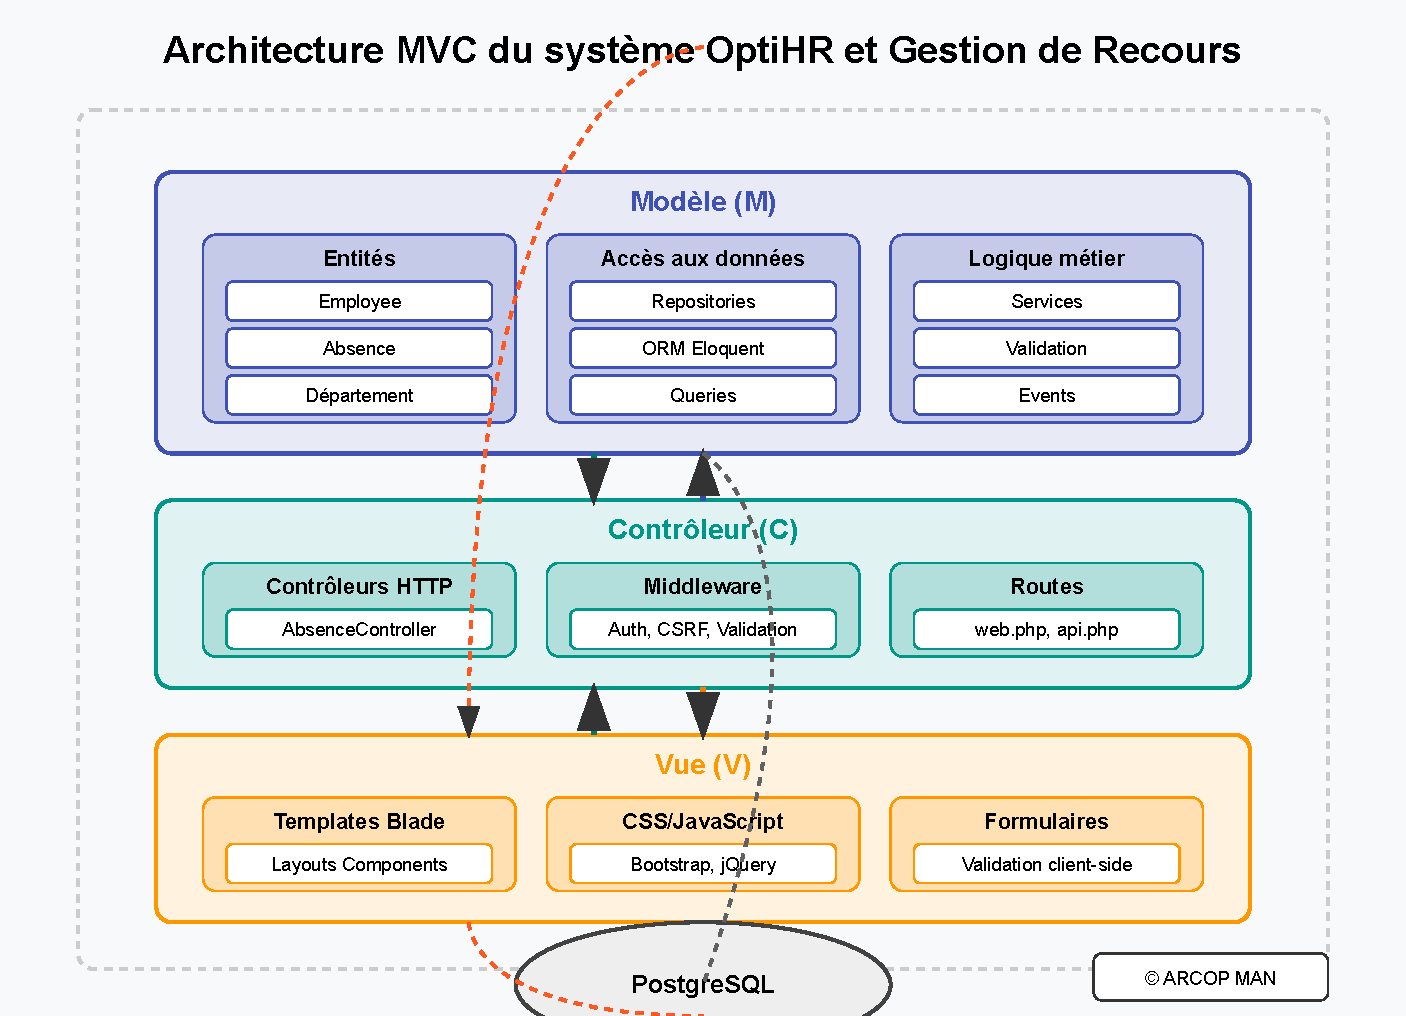
\includegraphics[width=0.9\textwidth]{images/diagrammes/architecture/architecture-couches.pdf}
    \caption{Architecture en couches du système OptiHR}
    \label{fig:architecture_couches}
\end{figure}

La figure \ref{fig:architecture_couches} illustre comment les différentes couches interagissent entre elles, avec un flux de données descendant pour les requêtes et ascendant pour les réponses. Les flèches représentent les dépendances entre les composants.

\subsection{Découpage modulaire du système}
Pour favoriser la maintenabilité et l'évolutivité, le système OptiHR est conçu selon une approche 
modulaire qui sépare les différentes préoccupations fonctionnelles:

\begin{enumerate}
    \item \textbf{Module d'authentification et autorisations}: Gestion des utilisateurs, des rôles et des permissions.
    \item \textbf{Module GRH}: Gestion des employés, des départements et de la documentation.
    \item \textbf{Module de gestion des absences}: Demandes de congés, workflow d'approbation et suivi.
    \item \textbf{Module de notifications}: Alertes système, notifications par email et notes de service.
    \item \textbf{Module documentaire}: Bulletins de paie, documents administratifs et archivage.
\end{enumerate}

\begin{figure}[H]
    \centering
    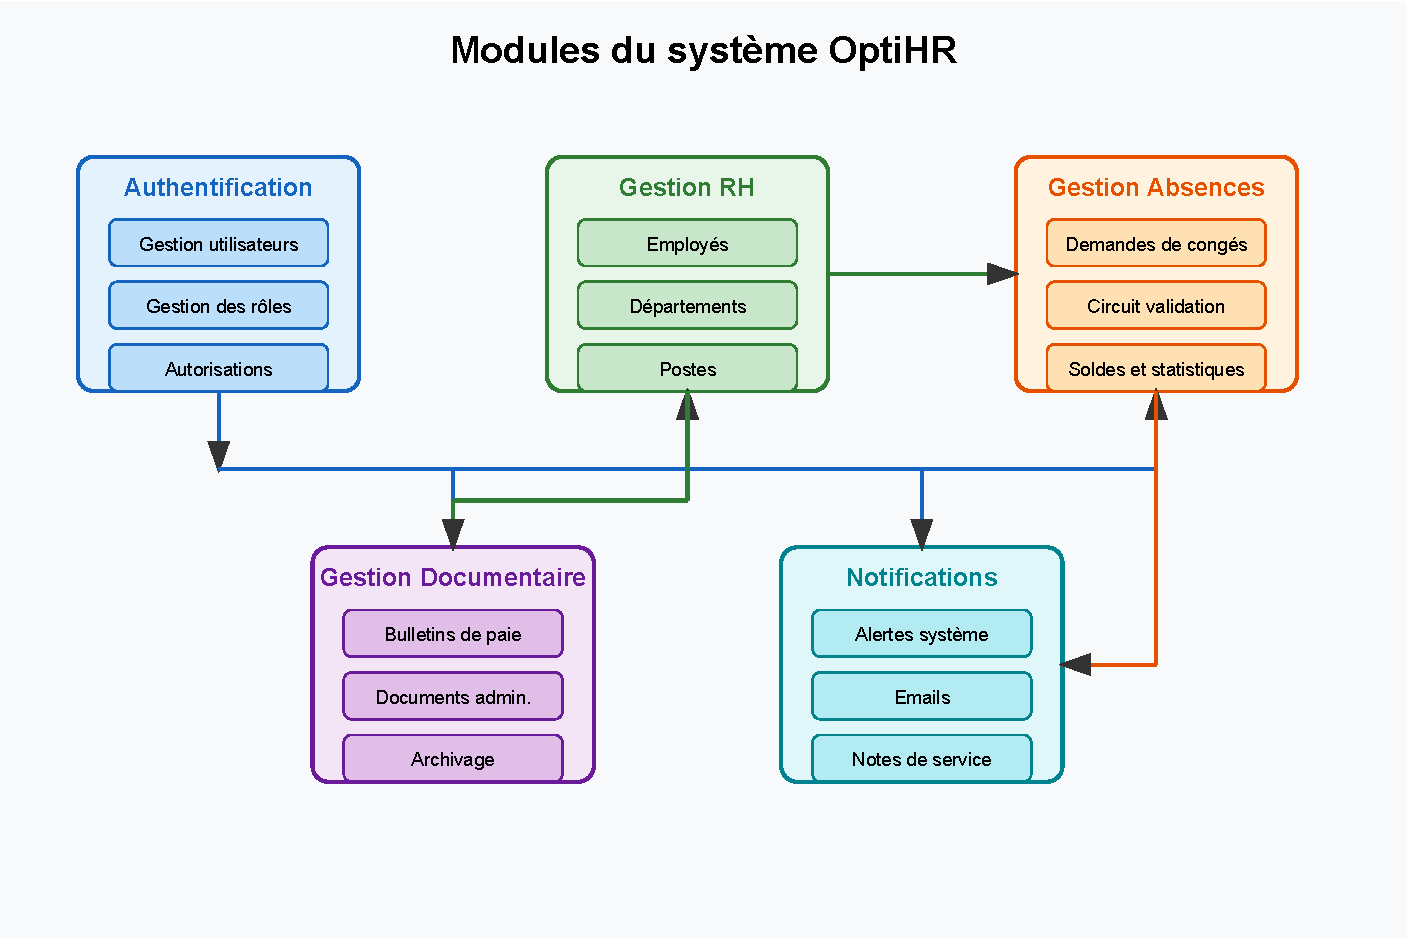
\includegraphics[width=0.9\textwidth]{images/diagrammes/architecture/modules-systeme.pdf}
    \caption{Organisation modulaire du système OptiHR}
    \label{fig:modules_systeme}
\end{figure}

Cette organisation modulaire, illustrée dans la figure \ref{fig:modules_systeme}, permet d'isoler les fonctionnalités 
et de faciliter les évolutions futures du système en minimisant les impacts entre modules.

\subsection{Flux de données et interactions}
Les interactions entre les composants suivent un flux standardisé qui garantit la cohérence des opérations
et facilite le débogage:

\begin{figure}[H]
    \centering
    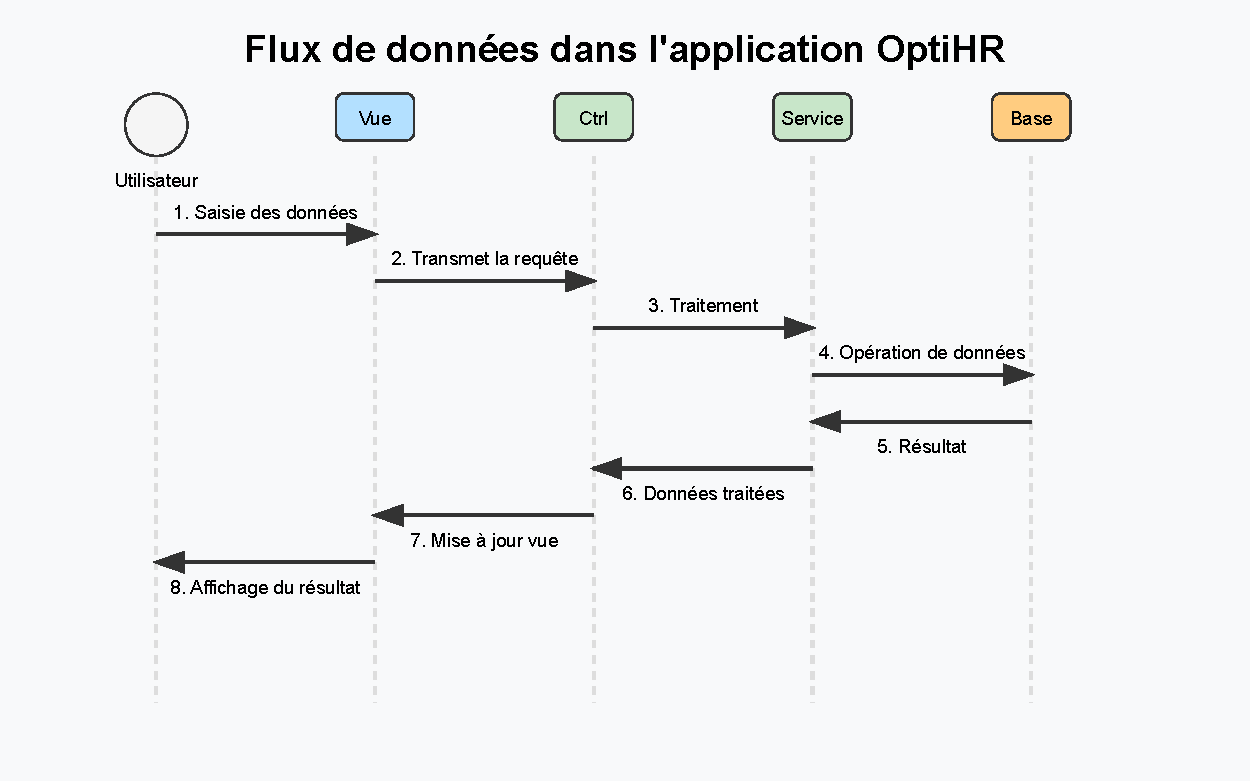
\includegraphics[width=0.9\textwidth]{images/diagrammes/architecture/flux-donnees.pdf}
    \caption{Flux de données dans l'application OptiHR}
    \label{fig:flux_donnees}
\end{figure}

Le diagramme de séquence (figure \ref{fig:flux_donnees}) détaille le parcours d'une requête typique à travers les différentes couches du système:

\begin{enumerate}
    \item L'utilisateur interagit avec l'interface (Vue)
    \item Les requêtes sont acheminées vers le Contrôleur approprié
    \item Le Contrôleur délègue le traitement aux Services
    \item Les Services manipulent les données via le Modèle
    \item Le Modèle interagit avec la base de données
    \item Les données sont remontées à travers les couches
    \item L'interface est mise à jour avec les résultats
    \item Le résultat final est affiché à l'utilisateur
\end{enumerate}

\subsection{Intégration avec les systèmes existants}
L'architecture du système OptiHR a été conçue pour s'intégrer harmonieusement avec l'infrastructure existante de l'ARCOP:

\begin{itemize}
    \item \textbf{Authentification unique}: Synchronisation possible avec l'annuaire d'entreprise
    \item \textbf{Import/Export}: Mécanismes d'échange de données avec les systèmes existants (Sage Paie, etc.)
    \item \textbf{API REST}: Interfaces programmables pour l'interopérabilité future avec d'autres applications
\end{itemize}

Cette approche garantit une intégration fluide dans l'écosystème applicatif de l'organisation tout en préservant l'autonomie du système.

\section{Modélisation des données}

\subsection{Dictionnaire de données}
Le dictionnaire de données ci-dessous détaille les structures de stockage avec leurs attributs, 
types, contraintes et descriptions. Cette documentation précise garantit l'intégrité et 
la cohérence des données manipulées par le système.

\renewcommand{\arraystretch}{1.3} % Améliore l'espacement du tableau

\begin{longtable}{|p{2.5cm}|p{3cm}|p{3cm}|p{3cm}|p{3cm}|}
    \hline
    \textbf{Table} & \textbf{Attribut} & \textbf{Type SQL} & \textbf{Contrainte} & \textbf{Description} \\
    \hline
    \endfirsthead

    \hline
    \textbf{Table} & \textbf{Attribut} & \textbf{Type SQL} & \textbf{Contrainte} & \textbf{Description} \\
    \hline
    \endhead

    % User
    \multirow{5}{*}{\textbf{Dacs}} & id & INT & PK, AUTO\_INCR. & Identifiant unique \\
    \cline{2-5}
    & reference & VARCHAR(50) & NOT NULL, UNIQUE & référence du marché \\
    \cline{2-5}
    & object & VARCHAR(255) & NOT NULL & Objet du marché \\
    \cline{2-5}
    \hline

    % Employee
    \multirow{5}{*}{\textbf{Decisions}} & id & INT & PK, AUTO\_INCR. & Identifiant unique \\
    \cline{2-5}
    & decision & VARCHAR(50) & NOT NULL & Décision \\
    \cline{2-5}
    & date & VARCHAR(50) & NOT NULL & Date de decision \\
    \cline{2-5}
    \hline

    % Department
    \multirow{3}{*}{\textbf{Applicants}} & id & INT & PK, AUTO\_INCR. & Identifiant unique \\
    \cline{2-5}
    & name & VARCHAR(100) & NOT NULL & Nom de lae la requérante \\
    \cline{2-5}
    & address &  VARCHAR(100) & NULL & Adresse \\
     \cline{2-5}
    & phone & VARCHAR(100) & NOT NULL, UNIQUE & Contact \\
    \cline{2-5}
     & nif & VARCHAR(100) & NOT NULL, UNIQUE & identification fiscal \\
    \cline{2-5}
    \hline

    % Role
    \multirow{2}{*}{\textbf{authorities}} & id & INT & PK, AUTO\_INCR. & Identifiant unique \\
    \cline{2-5}
    & name & VARCHAR(50) & NOT NULL & Nom de l'ac \\
    \hline

    % Permission
    \multirow{2}{*}{\textbf{appeals}} & id & INT & PK, AUTO\_INCR. & Identifiant unique \\
    \cline{2-5}
    & type & VARCHAR(50) & NOT NULL & type contestation \\
    \cline{2-5}
    & deposit\_date & DATE & NOT NULL & date dépôt \\
    \cline{2-5}
    & deposit\_hour & TIME & NOT NULL & heure dépôt \\
    \cline{2-5}
    & object & VARCHAR(255) & NOT NULL & objet du recours \\
    \cline{2-5}
    & day\_count & INT & NOT NULL & Durée de traitement \\
    \cline{2-5}
     & applicant\_id & INT & PK, FK(applicants.id) & Référence au requérant \\
     \cline{2-5}
     & dac\_id & INT & PK, FK(dacs.id) & Référence au marché \\
     \cline{2-5}
     & decision\_id & INT & PK, FK(decisions.id) & Référence au décision \\
     \cline{2-5}
     & authority\_id & INT & PK, FK(authorities.id) & Référence à l'autorité contractante \\
     \cline{2-5}
    & analyse\_status & VARCHAR & NOT NULL & Status de l'étude \\
    \hline


\end{longtable}
\begin{center}  
    \captionof{table}{Dictionnaire des données amélioré}
    \label{tab:table_dictionnaire_data_ameliore}  
\end{center}




\section{Modélisation objet}

\subsection{Diagramme de classes}
Le diagramme de classes constitue la représentation structurelle du système OptiHR. Il modélise les entités du domaine, leurs attributs et les relations qu'elles entretiennent entre elles. Cette modélisation répond aux besoins métier identifiés lors de la phase d'analyse et traduit fidèlement les processus de gestion des ressources humaines de l'ARCOP.

\begin{figure}[H]
    \centering
    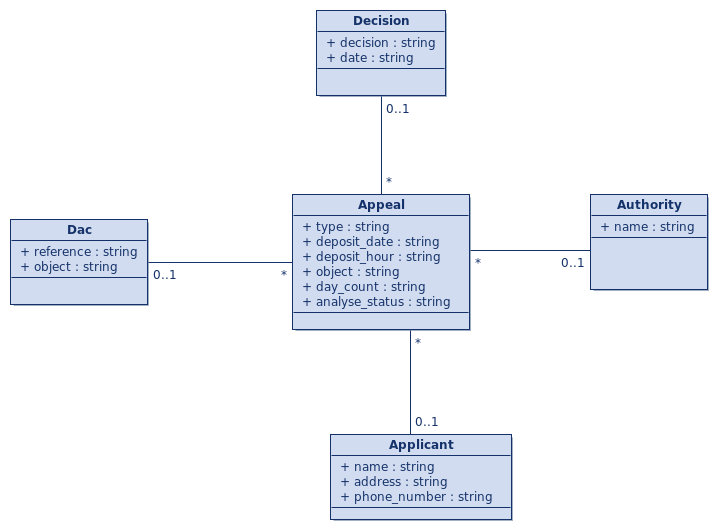
\includegraphics[width=\textwidth]{images/diagrammes/class/Diagramme de classe recours.png}
    \caption{Diagramme de classes des Recours}
    \label{fig:class_diagram_improved}
\end{figure}

La figure \ref{fig:class_diagram_improved} présente le diagramme de classes complet du système. Pour faciliter la compréhension, les entités sont regroupées par domaine fonctionnel:

\begin{itemize}
    \item \textbf{Domaine Utilisateur}: Gestion des accès et des permissions (User, Role, Permission)
    \item \textbf{Domaine Ressources Humaines}: Organisation et employés (Employee, Department, Job)
    \item \textbf{Domaine Opérationnel}: Activités et processus métier (Absence, Duty)
    \item \textbf{Domaine Documentaire}: Gestion des documents et médias (File, Image, Note, Decision)
\end{itemize}

\subsection{Relations et multiplicités}
Les relations entre les classes représentent les associations fonctionnelles au sein du système. Chaque relation est caractérisée par sa nature (association, composition, agrégation) et sa multiplicité, qui définit le nombre d'instances impliquées.

\begin{enumerate}
    \item \textbf{Appeal - Applicant} (n:1) : Un recours est déposé par un seul requérant, mais un requérant peut déposer plusieurs recours.
    
    \item \textbf{Appeal - Authority} (n:1) : Un recours peut être adressé à une seule autorité, mais une autorité peut recevoir plusieurs recours.
    
    \item \textbf{Appeal - Dac} (n:1) : Un recours peut être lié à un seul DAC (Dossier d'Appel d'Offres), mais un DAC peut concerner plusieurs recours.
    
    \item \textbf{Appeal - Decision} (n:1) : Chaque recours peut avoir une seule décision, et une décision est liée à plusieurs recours.
    
   
\end{enumerate}
